\documentclass{article}

\usepackage[poster]{staix_2026}

\usepackage[utf8]{inputenc}
\usepackage[T1]{fontenc}
\usepackage{hyperref}
\usepackage{booktabs}
\usepackage{graphicx}
\usepackage{amsmath,amssymb}

\title{Subject-Level Calibration Heterogeneity is Stable\\
  Across LLM Families and Scales: A Statistical Audit of MMLU}

\author{%
  Anonymous Author 1 \\
  Anonymous Institution \\
  \texttt{anon@anon.edu}
  \And
  Anonymous Author 2 \\
  Anonymous Institution \\
  \texttt{anon@anon.edu}
}

\begin{document}

\maketitle

% ============================================================
\section{Problem and Motivation}
% ============================================================

Calibration is nearly always evaluated as a single aggregate scalar---ECE, NLL,
or related---that aggregates over all subjects in a benchmark, obscuring whether
miscalibration is diffuse or concentrated in specific domains. We show the
concentration is structured: across seven instruction-tuned LLMs from three
families, the same subjects are stably worst-calibrated (college-level technical
content, professional law, virology) and best-calibrated (high-school Social
Sciences, applied/factual subjects), with subject-level ECE rankings correlated
at Spearman $\rho \in [0.80, 0.94]$ across all 15 pairs of larger models. This
stability points to task structure rather than any particular training pipeline.
The distinction matters for practice: if the pattern is stable, a subject-aware
audit run on one model generalizes to others, enabling portable pre-deployment
diagnostics without re-establishing baselines. Existing work has noted
calibration degrades on professional knowledge tasks \citep{xiong2024can},
but no prior work formally audits this structure---testing which subjects are
robustly miscalibrated, how much variance they explain, and whether the pattern
holds across models.

% ============================================================
\section{Approach}
% ============================================================

We apply a statistical audit framework to MMLU \citep{hendrycks2021measuring}
across seven instruction-tuned models: GPT-4o-mini, Llama-3-8B-Instruct, and
Qwen-2.5-\{0.5B, 1.5B, 3B, 7B, 14B\}-Instruct. Confidence is elicited via
softmax-renormalized token-level logprobs over \{A, B, C, D\}. The framework
combines: (i)~a three-level mixed-effects model decomposing calibration-gap
variance across questions, subjects, and domains; (ii)~isotonic reliability
curves and ECE per subject; (iii)~Benjamini--Hochberg FDR correction
\citep{bh1995} across 57 subjects per model; and (iv)~Spearman rank
correlations of subject-level ECE across all 21 model pairs. Question-level
covariates (word count, entropy, negation, option length) are included as fixed
effects to characterize which item features predict miscalibration.

% ============================================================
\section{Results}
% ============================================================

\paragraph{Structured heterogeneity.}
Between-subject variance accounts for 1.7--7.9\% of total calibration-gap
variance (ICC) across models---small in absolute terms but concentrated in
stable subject clusters. Gap ranges span $3.8$--$13.0\times$ from the best- to
worst-calibrated subject across the six larger models. At FDR $\alpha=0.05$,
five of six larger models reject all 57 subjects; the heterogeneity is
statistically real and robust to bin count and proper-scoring alternatives.

\paragraph{Stable patterns across models.}
Figure~\ref{fig:crossmodel} shows the 7$\times$7 Spearman rank correlation
matrix of subject-level ECE. Among the six models above 1B parameters, all 15
pairwise correlations fall in $[0.80, 0.94]$. Cross-family correlations
(GPT-4o-mini vs.\ Qwen-7B: 0.92; GPT-4o-mini vs.\ Qwen-14B: 0.91) are
comparable to the strongest within-family pairs, indicating the pattern is
task-driven rather than family-specific. Qwen-0.5B is the conspicuous
exception ($\rho \in [0.13, 0.20]$ with the others), driven by extreme
positional bias rather than genuine knowledge gaps.

\begin{figure}[h]
  \centering
  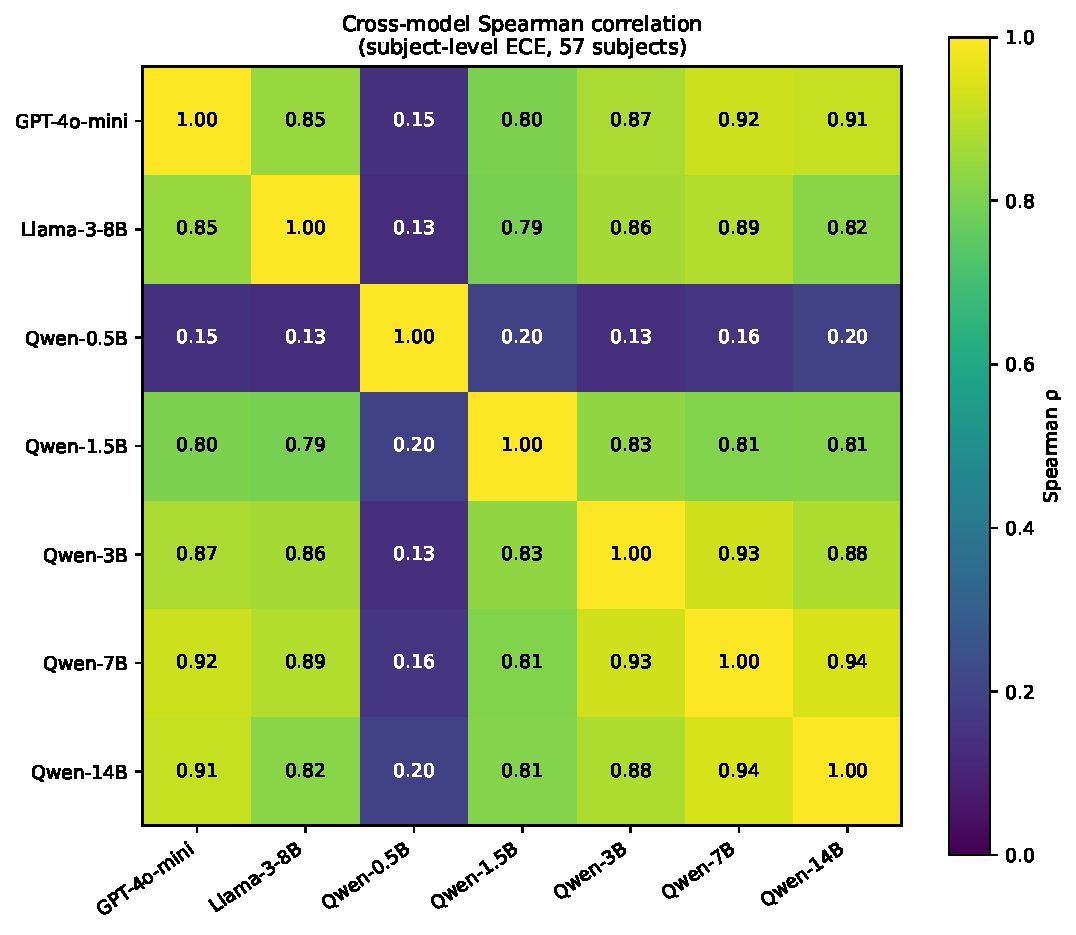
\includegraphics[width=0.62\columnwidth]{figures/cross_model_heatmap_7m.pdf}
  \caption{Spearman rank correlation of subject-level ECE across seven models.
  Among the six larger models, all 15 pairs fall in $[0.80, 0.94]$.
  Qwen-0.5B's low correlations reflect positional bias, not calibration structure.}
  \label{fig:crossmodel}
\end{figure}

\textbf{Worst-calibrated:} \texttt{virology} and \texttt{professional\_law}
land in the top-10 for every larger model; \texttt{abstract\_algebra},
\texttt{college\_mathematics}, and \texttt{machine\_learning} each appear for
four of six. \textbf{Best-calibrated:} \texttt{marketing} and
\texttt{high\_school\_psychology} are consistently at the other extreme.
The clearest organizing axes are specialization level (high-school vs.\
college content) and domain category (STEM vs.\ Social Sciences).
\textbf{Scaling:} within the Qwen family, the entropy coefficient on the
calibration gap grows monotonically with scale ($-0.004 \to +0.006 \to +0.029
\to +0.040$, significant at 7B and 14B), with confidence staying near
saturation as accuracy drops on harder items---a pattern also documented at
the aggregate level for RLHF-tuned models \citep{kadavath2022language,
nakkiran2025trained}.

% ============================================================
\section{Key Contribution}
% ============================================================

We provide the first formal statistical audit of subject-level calibration
heterogeneity in LLMs: variance decomposition, FDR-corrected rankings, and
cross-model stability testing across seven models from three families. The
finding that subject-level ECE rankings are highly stable across families and
scales has two practical consequences. First, the audit is portable: a deployer
can apply it to a new model and read off subject-level overconfidence directly,
using the recurring offenders (\texttt{professional\_law}, \texttt{virology},
college-level technical content) as a pre-deployment checklist. Second, the
stability provides the empirical precondition for subject-aware recalibration:
if the same subjects are consistently worst-calibrated, there is structure worth
correcting at the subject level rather than globally.

\bibliographystyle{plainnat}
\bibliography{references}

\end{document}
